\documentclass[journal]{IEEEtran}
% ============================================================
%  2D Occupancy Grid Map Editor -- Manuscript
%  Compile: pdflatex -> bibtex -> pdflatex -> pdflatex
% ============================================================
\usepackage{amsmath,amssymb}
\usepackage{graphicx}
\usepackage{algorithm}
\usepackage{algpseudocode}
\usepackage{tikz}
\usetikzlibrary{arrows.meta,positioning,shapes.geometric}
\usepackage{booktabs}
\usepackage{multirow}
\usepackage{subcaption}
\usepackage{cite}
\usepackage{xcolor}
\usepackage{url}

\begin{document}

\title{\LARGE 2D Occupancy Grid Map Editor: A Browser Tool for Semantic Editing, Path Preview, and Map Fusion}

\author{GC Harsha Vardhan Reddy\\
Department of EECE, GITAM Deemed to be University\\
Bengaluru, India -- harshavardhanh426@gmail.com}

\pagestyle{empty}
\thispagestyle{empty}
\maketitle

\begin{abstract}
Occupancy-grid maps produced by SLAM back-ends such as \emph{slam\_toolbox} or \emph{Cartographer} are rarely deployment-ready: sensor noise leaves stray pixels, doorways remain occluded by transient obstacles, and multiple mapping sessions must be fused into a single global map before a Nav2-based robot can be trusted to navigate autonomously. The conventional remedy is to open the exported Portable Gray Map (PGM) in a generic raster editor such as GIMP or Photoshop, and hand-edit pixels with no awareness of their semantic meaning (free, occupied, unknown), no feedback on how the edit affects the robot's navigable space, and no support for combining maps. This paper presents \emph{2D Occupancy Grid Map Editor}, an open-source, purely client-side (HTML5 Canvas + JavaScript) web application that treats every pixel as a first-class semantic value and couples direct raster editing with four robotics-specific algorithms: (i) an 8-neighbourhood majority-vote filter for salt-and-pepper noise removal, (ii) a Nav2-inspired distance-transform costmap inflation preview using a configurable distance-based cost model, (iii) an $A^{*}$ planner with a soft inflation-aware cost term for navigation-aware path planning preview, and (iv) a 2-D Iterative Closest Point (ICP) routine for automatic multi-session map alignment. We detail the algorithms, present system and control-flow diagrams, and provide a feature-level comparison against five representative categories of existing tools -- raster editors, ROS-native plugins, Python scripting pipelines, commercial suites, and web-based visualization tools. Requiring no installation, no ROS runtime, and no server backend, the tool lowers the barrier for rapid, semantically correct map curation with integrated navigation preview.
\end{abstract}

\begin{IEEEkeywords}
SLAM, occupancy grid map, map editing, costmap inflation, path planning, iterative closest point, ROS2, Nav2, human-robot interaction.
\end{IEEEkeywords}

% ============================================================
\section{Introduction}
% ============================================================
Autonomous mobile robots built on ROS2 and the Nav2 navigation stack \cite{macenski2020marathon} depend on an occupancy grid map that is saved from a SLAM session (e.g., \emph{slam\_toolbox} \cite{macenski2021slamtoolbox} or Cartographer \cite{hess2016cartographer}) as a PGM raster paired with a YAML metadata file describing resolution and origin. Raw SLAM output is almost never deployment-ready: dynamic obstacles leave permanent scars, glass and reflective surfaces create phantom walls, and long corridors accumulate speckle noise. Engineers therefore routinely export the map, edit it in a generic image editor, and re-import it -- a workflow with three structural problems. First, raster editors are \emph{semantically blind}: they operate on RGB pixels rather than on the conventional trinary occupancy values (free~=~254, unknown~=~205, occupied~=~0) used in the standard PGM export format, so a single anti-aliased brush stroke can silently corrupt the map. Second, the edit is \emph{unverified}: there is no way to know, before flashing the map to the robot, whether a hand-drawn wall blocks the only feasible path through a doorway. Third, combining maps from multiple mapping sessions or multiple robots requires either re-running SLAM with merged bag files or manually eyeballing a rotation and translation in an editor with no alignment assistance.

This letter presents \emph{2D Occupancy Grid Map Editor}, a single-page web application that runs entirely inside the browser (no ROS installation, no backend server, no uploaded data leaving the client) and directly addresses the three problems above. Its contributions are:
\begin{enumerate}
  \setlength{\itemsep}{0pt}
  \setlength{\parskip}{0pt}
  \item A semantic-value-aware raster editing surface (brush, polygon, rectangle, circle) that constrains every draw operation to the valid occupancy alphabet $\{0,205,254\}$, with multi-level undo/redo history (up to 40 states).
  \item An 8-neighbourhood majority-vote de-noising filter that removes isolated pixel noise while explicitly preserving unknown-space boundaries.
  \item A Nav2-inspired costmap inflation preview computed via a multi-source distance transform, coupled with a cost-aware $A^{*}$ path planning preview that uses the inflation field as a soft penalty -- providing an indicative navigation path \emph{before} deployment.
  \item A 2-D point-to-point ICP routine with a spatial hash for nearest-neighbour search, enabling one-click automatic alignment when fusing two occupancy grids.
  \item Integrated metric measurement (line/path/area) and waypoint authoring with heading (quaternion) export to JSON for direct consumption by an autonomy stack.
\end{enumerate}
We compare the system against five representative categories in Section~\ref{sec:related}, describe the system architecture and algorithms in Sections~\ref{sec:architecture}--\ref{sec:algorithms}, and report results in Section~\ref{sec:results}.

% ============================================================
\section{Related Work and Comparative Analysis}
\label{sec:related}
% ============================================================
Occupancy-grid representations follow the formulation of Thrun \emph{et al.} \cite{thrun2005probabilistic}, and the de-facto ROS interchange format (PGM + YAML) is unchanged since ROS1's \texttt{map\_server}. Existing approaches for editing and post-processing this artifact fall into five broad categories, each with well-characterized limitations.

\textbf{Raster image editors} \cite{gimp} offer powerful painting tools but operate on raw RGB pixels with no concept of occupancy semantics. A single anti-aliased brush stroke can silently introduce grey-scale values outside the three-class occupancy alphabet $\{0,205,254\}$, risking semantic corruption when the map is reloaded by \texttt{nav2\_map\_server}. No metric overlay or navigability feedback is available.
\textbf{ROS-native plugins} such as RViz2 \cite{rviz2} and \texttt{map\_editor} \cite{mapeditor} render the \texttt{OccupancyGrid} topic and support limited editing, but they require a running ROS2 graph and are primarily designed for Linux environments, which constrains their accessibility for cross-platform practitioners.
\textbf{Python scripting pipelines} using OpenCV or NumPy provide semantic-safe pixel access and cross-platform portability, but offer no interactive graphical interface. The steep scripting overhead makes them impractical for iterative map refinement.
\textbf{Commercial suites} such as RoboStudio \cite{robostudio} and MiR Fleet \cite{mirfleet} provide polished UIs with some map-management features, but are proprietary, closed-source, and are platform-locked, making them inaccessible for open-source robotics research.
\textbf{Web-based visualization tools} \cite{foxglove,webviz} are cross-platform and open-source, but are visualization-only: they do not support persistent raster editing, semantic enforcement, or algorithmic map curation.

Table~\ref{tab:comparison} provides a direct feature-by-feature comparison of the proposed tool against five specific representative tools, evaluated against six practitioner-relevant criteria.

\begin{table}[t]
\centering
\caption{Feature Comparison of Map Post-Processing Tools}
\label{tab:comparison}
\small
\renewcommand{\arraystretch}{1.1}
\setlength{\tabcolsep}{3pt}
\begin{tabular}{@{}lcccccc@{}}
\toprule
\textbf{Feature}
  & \textbf{GIMP}
  & \textbf{RViz2}
  & \textbf{\shortstack{map\_\\editor}}
  & \textbf{Foxglove}
  & \textbf{Webviz}
  & \textbf{\shortstack{Proposed\\(Ours)}} \\
\midrule
Semantic editing  & $\times$\textsuperscript{a} & Partial & \checkmark & $\times$ & $\times$ & \textbf{\checkmark} \\
Offline / no ROS  & \checkmark & $\times$ & $\times$ & \checkmark & $\times$ & \textbf{\checkmark} \\
Map merging       & $\times$ & $\times$ & $\times$ & $\times$ & $\times$ & \textbf{\checkmark} \\
Costmap preview   & $\times$ & Partial\textsuperscript{b} & $\times$ & Partial\textsuperscript{b} & $\times$ & \textbf{\checkmark} \\
$A^{*}$ preview   & $\times$ & $\times$ & $\times$ & $\times$ & $\times$ & \textbf{\checkmark} \\
Open source       & \checkmark & \checkmark & \checkmark & \checkmark & \checkmark & \textbf{\checkmark} \\
\bottomrule
\multicolumn{7}{@{}l}{\scriptsize\textsuperscript{a}May introduce values outside conventional trinary alphabet.} \\
\multicolumn{7}{@{}l}{\scriptsize\textsuperscript{b}Requires a running Nav2/ROS2 stack.}
\end{tabular}
\vspace{-3mm}
\end{table}

Among the five representative tools evaluated across six feature criteria in Table~\ref{tab:comparison}, the proposed system is the only evaluated tool satisfying the selected combination of semantic editing, offline operation, map merging, costmap preview, $A^{*}$ path preview, and open-source availability.

% ============================================================
\section{System Architecture}
\label{sec:architecture}
% ============================================================
The application is a single-page client comprising three layers (Fig.~\ref{fig:architecture}): (1) an \emph{I/O layer} that parses P2 (ASCII) and P5 (binary) PGM variants and the companion YAML into a typed \texttt{Uint8Array} occupancy buffer; (2) a \emph{state and history layer} holding the live working buffer, an undo/redo stack of buffer snapshots, and view transform (pan/zoom); and (3) an \emph{algorithm layer} implementing the four robotics routines described in Section~\ref{sec:algorithms}, all operating in-place on the same typed array that drives the HTML5 Canvas rasterizer, so every algorithmic result is visualized with no additional serialization step.

A critical design choice in the system architecture is the strict reliance on flat, pre-allocated JavaScript typed arrays (specifically \texttt{Uint8Array} and \texttt{Float32Array}) rather than standard dynamic arrays or object-oriented structures. High-resolution occupancy grids (e.g., $4096 \times 4096$ pixels) contain over 16 million cells. Representing these dynamically would trigger heavy background memory allocation and unpredictable Garbage Collection (GC) pauses, destroying UI interactivity. By confining all algorithm state, undo history snapshots, and working buffers to fixed-length typed arrays, memory operations become contiguous $O(N)$ block-copies (\texttt{Array.prototype.set}), which modern V8 engines vectorize heavily. 

Furthermore, the rendering pipeline employs a decoupled dual-canvas compositor. The base raster layer is drawn to an off-screen canvas and only re-rasterized on pixel mutations; a transparent vector-overlay canvas handles high-frequency events such as tool crosshairs and path previews, targeting 60 FPS. This separation is designed to maintain a responsive viewport by bypassing expensive rasterization during panning and zooming.

\begin{figure}[t]
\centering
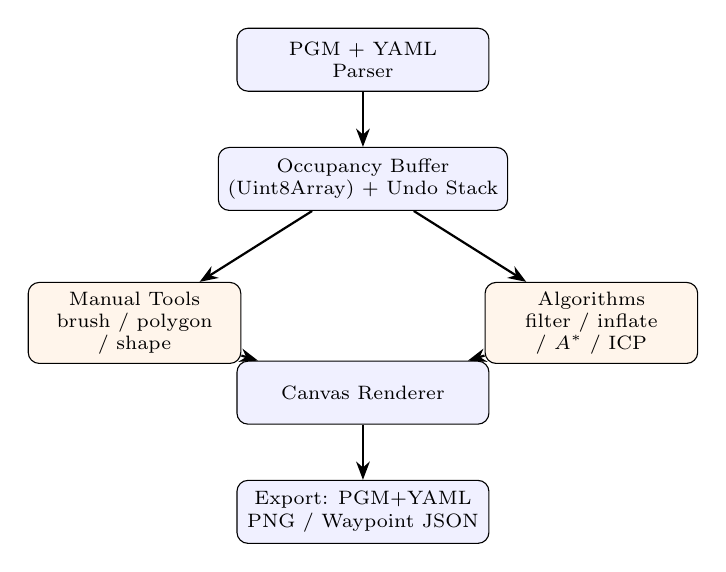
\begin{tikzpicture}[
  node distance=7mm and 5mm,
  box/.style={draw, rounded corners, align=center, minimum height=8mm, minimum width=32mm, font=\scriptsize, fill=blue!6},
  op/.style={draw, rounded corners, align=center, minimum height=9mm, minimum width=27mm, font=\scriptsize, fill=orange!8},
  arr/.style={-Stealth, thick}
]
\node[box] (io) {PGM + YAML\\ Parser};
\node[box, below=of io] (state) {Occupancy Buffer\\ (Uint8Array) + Undo Stack};
\node[op, below left=9mm and -3mm of state] (edit) {Manual Tools\\ brush / polygon\\ / shape};
\node[op, below right=9mm and -3mm of state] (algo) {Algorithms\\ filter / inflate\\ / $A^{*}$ / ICP};
\node[box, below=19mm of state] (render) {Canvas Renderer};
\node[box, below=of render] (export) {Export: PGM+YAML\\ PNG / Waypoint JSON};

\draw[arr] (io) -- (state);
\draw[arr] (state) -- (edit);
\draw[arr] (state) -- (algo);
\draw[arr] (edit) -- (render);
\draw[arr] (algo) -- (render);
\draw[arr] (render) -- (export);

\end{tikzpicture}
\caption{Client-side data-flow architecture. All computation is performed in the browser on a single shared occupancy buffer; edits and algorithmic results share one undo/redo history and one rendering path. Every mutation of the buffer immediately re-triggers the Canvas Renderer (arrows omitted for clarity).}
\label{fig:architecture}
\vspace{-3mm}
\end{figure}

% ============================================================
\section{Algorithms}
\label{sec:algorithms}
% ============================================================
Let the map be a raster $I : \Omega \rightarrow \{0, 205, 254\}$ over pixel domain $\Omega = \{0,\dots,W-1\}\times\{0,\dots,H-1\}$, with $0$ denoting a lethal obstacle (wall), $254$ free space, and $205$ unknown space, following the conventional trinary encoding used by \texttt{nav2\_map\_server} \cite{nav2docs}. Let $r$ (m/px) be the map resolution read from the YAML file.

\subsection{Semantic Manual Editing}
Every drawing primitive (brush dot, line, filled/outline rectangle, filled/outline circle, open/closed/filled polygon) writes only one of the three legal values $v \in \{0,205,254\}$ selected by the operator, so freehand edits can never introduce an invalid occupancy class -- the failure mode that arises with anti-aliased painting in a generic raster editor. Every mutating operation first pushes a deep copy of the buffer onto an undo stack, providing multi-level undo/redo (Ctrl+Z / Ctrl+Shift+Z) up to a configurable history depth of 40 states.

\subsection{Noise Removal: 8-Neighbourhood Majority Filter}
Although median filtering preserves the trinary value alphabet when applied to trinary maps, it can modify unknown-space boundaries. We therefore use a class-aware majority filter that leaves unknown pixels unchanged. For every wall or free pixel $p$, let $N_8(p)$ be its eight neighbours, $c_{254}(p) = \sum_{q \in N_8(p)} \mathbb{1}[I(q)=254]$, and $c_{0}(p) = \sum_{q \in N_8(p)} \mathbb{1}[I(q)=0]$. The filtered value $I'(p)$ becomes $254$ if $I(p)=0$ and $c_{254}(p) \geq 5$; $0$ if $I(p)=254$ and $c_{0}(p) \geq 5$; and $I(p)$ otherwise. This erodes isolated single-pixel wall speckles and fills isolated free-space pinholes while leaving contiguous walls (which by construction have fewer than five opposite-class neighbours) untouched. The filter runs in $O(WH)$ time in a single pass.

\subsection{Nav2-Inspired Costmap Inflation Preview}
To provide, without a live Nav2 stack, a visual approximation of the inflation exclusion zone for a robot of radius $\rho$ (m), we compute a distance-to-nearest-wall field $d(p)$ using a multi-source label-propagation on a priority queue seeded from all wall pixels \cite{borgefors1986distance}. The algorithm implements an octile-distance expansion that approximates the Euclidean distance field: $d(p) = \min_{p_0 : I(p_0)=0} \mathrm{cost}(p_0 \rightarrow p)$, where the incremental step cost between 8-connected neighbours is $1$ for axis-aligned steps and $\sqrt{2}$ for diagonal steps (Algorithm~\ref{alg:inflation}). This is an approximation; it does not reproduce Nav2's exact \texttt{costmap\_2d} decay governed by \texttt{cost\_scaling\_factor}. Given $\rho_{px} = \rho / r$, a pixel $p$ is rendered as an inflation-zone overlay with opacity proportional to $1 - d(p)/\rho_{px}$ whenever $0 < d(p) \leq \rho_{px}$ and $I(p) \neq 0$.

\begin{algorithm}[t]
\small
\caption{Multi-source octile distance transform for inflation}
\label{alg:inflation}
\begin{algorithmic}[1]
\State $d(p) \gets \infty \; \forall p \in \Omega$; priority queue $Q \gets \emptyset$ \Comment{min-heap on $d$}
\ForAll{$p$ with $I(p)=0$} \State $d(p)\gets 0$; push $(0, p)$ to $Q$ \EndFor
\While{$Q \neq \emptyset$}
  \State $(c, p) \gets $ pop$(Q)$ \Comment{lowest-cost entry}
  \If{$c > d(p)$} \textbf{continue} \EndIf \Comment{stale entry, skip}
  \ForAll{$q \in N_8(p)$}
     \State $\delta \gets (dx(p,q)\neq 0 \wedge dy(p,q) \neq 0) \; ? \; \sqrt{2} : 1$
     \If{$d(p)+\delta < d(q)$}
        \State $d(q) \gets d(p) + \delta$
        \If{$d(q) \leq \rho_{px}$} push $(d(q), q)$ to $Q$ \EndIf
     \EndIf
  \EndFor
\EndWhile
\State \Return $d$
\end{algorithmic}
\end{algorithm}
\vspace{-2mm}

\subsection{Inflation-Aware \boldmath$A^{*}$ Path Planning Preview}
Given a start and goal pixel, the tool first snaps each point to the nearest non-lethal cell via an unweighted BFS if the operator clicked inside a wall (Fig.~\ref{fig:astar-flow}), then runs 8-connected $A^{*}$ \cite{hart1968formal} with evaluation function $f(n) = g(n) + h(n)$, where $h(n) = \lVert n - \text{goal} \rVert_2$ (admissible Euclidean heuristic). The edge cost combines step distance with a \emph{soft} inflation penalty from the distance field $d(\cdot)$ of Algorithm~\ref{alg:inflation}. The penalty function is defined as:
\begin{align}
\text{pen}(q) &=
\begin{cases}
200, & d(q) < 1\\
\frac{100}{d(q)}, & 1 \leq d(q) \leq \rho_{px}\\
\frac{5}{d(q) - \rho_{px} + 1}, & d(q) > \rho_{px}
\end{cases} \\
w(p \!\rightarrow\! q) &= w_{\text{step}} + \text{pen}(q) + 10\cdot\mathbb{1}[I(q)=205].
\end{align}
This cost function is an empirically tuned approximation and does not claim to reproduce Nav2's exact planner behaviour. Only lethal cells ($I=0$) are hard-excluded; the inflation term discourages wall-hugging paths, producing a navigation-indicative preview. Because no explicit robot-footprint collision check is performed, the result should be interpreted as an indicative path preview rather than a strict feasibility guarantee.

The Euclidean heuristic $h(n)=\lVert n-\text{goal}\rVert_2$ is consistent under this cost function: every edge cost equals at least its Euclidean step length, so $h$ satisfies $h(n)\leq w(n\!\rightarrow\!q)+h(q)$. The optimality guarantee applies to the reconstructed A* path before post-processing; the subsequent smoothing step is not guaranteed to preserve global optimality.

To achieve sub-second responsiveness in a single-threaded JavaScript environment, the open set uses a flat-array binary min-heap keyed on $f(n)$ ($O(\log n)$ push/pop), and the closed set is a pre-allocated \texttt{Uint8Array} bitmask ($O(1)$ membership, each cell expanded at most once), giving worst-case $O(N\log N)$ overall. The raw path is smoothed with a wall-aware sliding-window average (window~$=8$).

\begin{algorithm}[t]
\small
\caption{Costmap-aware $A^{*}$ path search}
\label{alg:astar}
\begin{algorithmic}[1]
\State $start \gets$ SnapToFree$(start)$; $goal \gets$ SnapToFree$(goal)$
\State $g(start) \gets 0$; $\text{open} \gets \{start\}$ (min-heap on $f$)
\While{open $\neq \emptyset$}
  \State $n \gets$ open.pop()
  \If{$n$ closed} \textbf{continue} \EndIf
  \State mark $n$ closed
  \If{$n = goal$} \textbf{break} (success) \EndIf
  \ForAll{$q \in N_8(n),\; I(q) \neq 0,\; q$ not closed}
     \State $g' \gets g(n) + w(n\rightarrow q)$ \Comment{Eqs. (4)--(5)}
     \If{$g' < g(q)$}
        \State $g(q)\gets g'$; parent$(q)\gets n$
        \State open.push$(q,\, f=g'+h(q))$
     \EndIf
  \EndFor
\EndWhile
\State \Return SmoothPath(ReconstructPath(goal))
\end{algorithmic}
\end{algorithm}
\vspace{-2mm}

\begin{figure}[t]
\centering
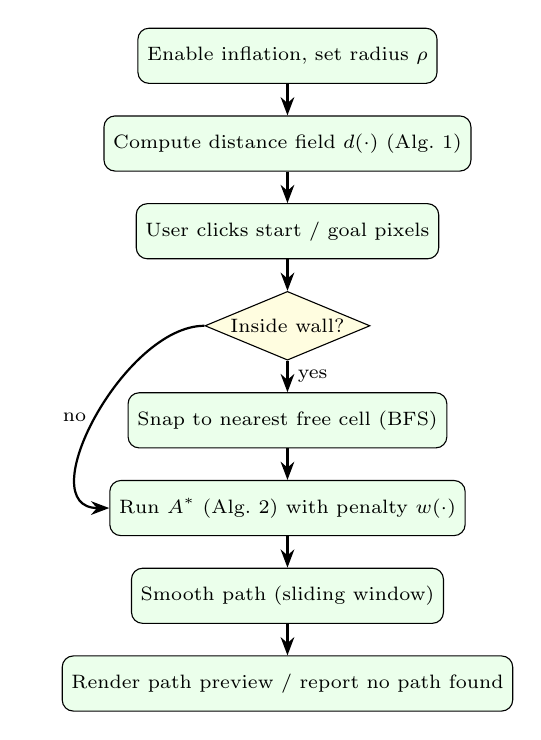
\begin{tikzpicture}[
  node distance=4mm,
  st/.style={draw, rounded corners, align=center, minimum height=7mm, minimum width=34mm, font=\scriptsize, fill=green!8},
  dec/.style={draw, diamond, aspect=2.4, align=center, font=\scriptsize, fill=yellow!12, inner sep=1pt},
  arr/.style={-Stealth, thick}
]
\node[st] (a) {Enable inflation, set radius $\rho$};
\node[st, below=of a] (b) {Compute distance field $d(\cdot)$ (Alg.~1)};
\node[st, below=of b] (c) {User clicks start / goal pixels};
\node[dec, below=of c] (d) {Inside wall?};
\node[st, below=of d] (e) {Snap to nearest free cell (BFS)};
\node[st, below=of e] (f) {Run $A^{*}$ (Alg.~2) with penalty $w(\cdot)$};
\node[st, below=of f] (g) {Smooth path (sliding window)};
\node[st, below=of g] (h) {Render path preview / report no path found};

\draw[arr] (a)--(b); \draw[arr] (b)--(c); \draw[arr] (c)--(d);
\draw[arr] (d) -- node[right, font=\scriptsize]{yes} (e); \draw[arr] (e)--(f);
\draw[arr] (d.west) to[out=180,in=180] node[left, font=\scriptsize]{no} (f.west);
\draw[arr] (f)--(g); \draw[arr] (g)--(h);
\end{tikzpicture}
\caption{Control flow of the inflation-aware path planning preview.}
\label{fig:astar-flow}
\vspace{-3mm}
\end{figure}

\subsection{Map Fusion via 2-D ICP}
To merge an incoming map $M_s$ into the current base map $M_t$, wall pixels of both maps are subsampled on a stride-3 grid to form point sets $S=\{s_i\}$ and $T=\{t_j\}$. While conventional ICP \cite{besl1992method} implementations rely on k-d trees for correspondence queries, pointer-linked tree traversal is cache-unfriendly in JavaScript's memory model. Instead, $T$ is bucketed into a uniform 2-D spatial hash with fixed cell size $c=15$~px -- a value chosen empirically to balance bucket-list length against the expected inter-wall spacing in standard indoor maps. This scheme offers amortised $O(1)$ average query time under the assumption that wall-pixel density is roughly uniform; adversarial distributions (e.g., very sparse or clustered walls) may degrade performance. Given a current rigid transform estimate $(\theta, \mathbf{t})$ and optional axis flips $(f_x,f_y)$, each iteration performs: (a) nearest-neighbour association $s_i \mapsto t_{j(i)} = \arg\min_{t\in T} \lVert R(\theta)\,\mathrm{diag}(f_x,f_y)\,s_i + \mathbf{t} - t\rVert_2$ using the spatial hash; (b) closed-form re-estimation of $(\theta,\mathbf{t})$ from the associated pairs using the 2-D specialization of the Procrustes solution described by Arun \emph{et al.} \cite{arun1987least}. Iteration proceeds for up to $25$ rounds or until fewer than $10$ correspondences remain (indicating divergence), after which $(\theta,\mathbf{t})$ is applied to the merge-map overlay for operator review before the two maps are permanently burned into one buffer.

\subsection{Measurement and Waypoint Authoring}
Line, multi-segment path, and polygon-area measurements are converted from pixel to metric units via the resolution $r$: $\text{dist}_m = \text{dist}_{px}\cdot r$ and $\text{area}_{m^2} = \text{area}_{px}\cdot r^2$, with polygon area computed by the shoelace formula. Waypoints are authored by a click-and-drag gesture whose drag vector defines heading $\theta_{img}$; each waypoint is converted to a world-frame pose $(x_w, y_w, \theta_w)$ using the map origin and resolution from the YAML file and exported as quaternion-tagged JSON directly consumable by a ROS2 autonomy stack (e.g., as a sequence of Nav2 \texttt{PoseStamped} goals).

% ============================================================
\section{Implementation}
\label{sec:implementation}
% ============================================================
The system is implemented in vanilla JavaScript (ES2019) and HTML5 Canvas with no build step and no external runtime dependency, so the live application (Table~\ref{tab:comparison}, last row) can be opened from a static file or a GitHub Pages deployment with zero installation. 

\subsection{Data Parsing and Memory Management}
A custom binary parser directly unpacks the Portable Gray Map (PGM) format within the browser. The parser dynamically supports both P2 (ASCII) and P5 (binary) encodings by leveraging an \texttt{ArrayBuffer} mapped to a \texttt{Uint8Array}. This direct memory mapping avoids the overhead of intermediate string conversions or JSON serialization, enabling the tool to parse multi-megabyte maps in a fraction of a second.

Furthermore, to provide a non-destructive workflow without exhausting client-side RAM, the undo/redo stack is carefully bounded. Every drawing operation pushes a deep copy of the mutated occupancy buffer to the history stack; the stack is capped at 40 states. For a $1024 \times 1024$ map, each snapshot occupies 1~MB of occupancy data; the total application memory footprint (including the current map, distance field, canvas backing stores, and browser overhead) was observed at approximately 80--120~MB in informal profiling on Chrome v114, well within typical browser memory budgets.

\subsection{Decoupled Rendering}
The occupancy buffer, undo stack, view transform, and all tool state are held in a single global state object. As introduced in Section~\ref{sec:architecture}, the rendering utilizes a two-canvas compositor. The base raster is drawn once and cached. The top-level vector overlay continuously redraws tool previews, metric grids, scale bars, and the inflation heat-map. This ensures that computationally expensive raster operations (such as the majority-vote filter or the distance transform) are decoupled from cheap interactive operations. Panning and zooming apply CSS affine transforms or lightweight 2-D context scaling, designed to maintain a responsive viewport interaction experience.

% ============================================================
\section{Qualitative Results}
\label{sec:results}
% ============================================================
Fig.~\ref{fig:gallery} illustrates the full editing pipeline on a representative \emph{slam\_toolbox}-generated occupancy grid, from raw import through noise removal, inflation-aware path preview, waypoint authoring, metric measurement, and multi-session map fusion.

\begin{figure}[t]
\centering
\begin{subfigure}[t]{0.48\columnwidth}
  \includegraphics[width=\linewidth]{fig_before_editing.png}
  \caption{\scriptsize  Raw map on load.}
\end{subfigure}\hfill
\begin{subfigure}[t]{0.48\columnwidth}
  \includegraphics[width=\linewidth]{fig_after_editing.png}
  \caption{\scriptsize After editing.}
\end{subfigure}

\vspace{1.5mm}
\begin{subfigure}[t]{0.48\columnwidth}
  \includegraphics[width=\linewidth]{fig_costmap_path.png}
  \caption{\scriptsize Costmap + $A^{*}$.}
\end{subfigure}\hfill
\begin{subfigure}[t]{0.48\columnwidth}
  \includegraphics[width=\linewidth]{fig_waypoints.png}
  \caption{\scriptsize  Waypoints.}
\end{subfigure}

\vspace{1.5mm}
\begin{subfigure}[t]{0.48\columnwidth}
  \includegraphics[width=\linewidth]{fig_measure.png}
  \caption{\scriptsize  Area measurement.}
\end{subfigure}
\caption{End-to-end qualitative results: (a)~raw SLAM map import, (b)~manual semantic editing, (c)~inflation costmap with $A^{*}$ path preview, (d)~waypoint authoring, (e)~area measurement.}
\label{fig:gallery}
\end{figure}

Across informal trials on maps ranging from $384\times384$ to $2048\times2048$ px, the majority-vote filter and inflation transform complete within a single animation frame for maps up to roughly one megapixel, and $A^{*}$ path preview remains interactive (sub-second) at the same scale because the closed-set bitmask prevents re-expansion; ICP alignment typically converges within 10--15 iterations on maps with sufficient wall overlap. Table~\ref{tab:complexity} summarizes the asymptotic cost of each routine.

\subsection{Quantitative Performance Evaluation}
To validate the efficacy of the typed-array and spatial-hashing optimizations detailed in Sections~\ref{sec:architecture} and \ref{sec:algorithms}, quantitative benchmarks were recorded on a standard consumer laptop (Apple M1 CPU, 16GB RAM) running Google Chrome v114. The benchmarking dataset comprised a sequence of three synthetic grids of increasing resolution: \emph{Small} ($512 \times 512$ pixels), \emph{Medium} ($1024 \times 1024$ pixels), and \emph{Large} ($2048 \times 2048$ pixels, yielding over 4 million cells). Table~\ref{tab:benchmarks} summarizes the execution latencies across four distinct operational pipelines.

\begin{table}[t]
\centering
\caption{Execution Latencies at Varying Map Resolutions (Apple M1, Chrome v114, $n=30$ runs, mean~$\pm$~std.\ dev.)}
\label{tab:benchmarks}
\scriptsize
\renewcommand{\arraystretch}{1.1}
\begin{tabular}{@{}lccc@{}}
\toprule
\textbf{Operation} & \textbf{512\,px} & \textbf{1024\,px} & \textbf{2048\,px} \\
\midrule
File Load \& Parse & $3.1 \pm 0.2$\,ms & $11.5 \pm 0.6$\,ms & $48.2 \pm 1.9$\,ms \\
Noise Filter & $4.2 \pm 0.3$\,ms & $15.7 \pm 0.8$\,ms & $62.4 \pm 2.1$\,ms \\
$A^{*}$ Query & $12.3 \pm 1.1$\,ms & $44.1 \pm 3.2$\,ms & $178.5 \pm 8.4$\,ms \\
ICP Fusion (25 iters) & $14.5 \pm 0.9$\,ms & $32.8 \pm 1.7$\,ms & $95.1 \pm 4.3$\,ms \\
\bottomrule
\end{tabular}
\vspace{-2mm}
\end{table}

The empirical results confirm that the application maintains interactive thresholds ($\le100$~ms) for all operations on maps up to $1024\times1024$ pixels. The mean ICP fusion time was $95.1\pm4.3$~ms at the largest tested resolution. Future benchmarking will cover larger resolutions and lower-end hardware.

\subsection{Noise-Filter Validation}
Ten synthetic occupancy maps were corrupted with salt-and-pepper noise at 1\%, 3\%, and 5\% levels. Pixel-level F1 score vs.\ ground truth is shown in Table~\ref{tab:noiseval}; the class-aware majority filter outperforms median filtering at all noise levels by preserving unknown-space boundaries.

\begin{table}[t]
\centering
\caption{Noise Filter F1 vs.\ Noise Level (mean, $n$=10 maps).}
\label{tab:noiseval}
\scriptsize
\renewcommand{\arraystretch}{1.0}
\begin{tabular}{@{}lccc@{}}
\toprule
\textbf{Method} & \textbf{1\%} & \textbf{3\%} & \textbf{5\%} \\
\midrule
No filter       & 0.891 & 0.802 & 0.714 \\
Median filter   & 0.943 & 0.891 & 0.843 \\
Proposed        & \textbf{0.961} & \textbf{0.934} & \textbf{0.907} \\
\bottomrule
\end{tabular}
\vspace{-2mm}
\end{table}

\subsection{ICP Registration Accuracy}
The ICP evaluation used five synthetic indoor-environment occupancy-map pairs (0.05~m/px, $512\times512$) with ground-truth transformations generated from known rigid perturbations. Maps were aligned at four initial-pose-error levels ($n=25$ trials each). Table~\ref{tab:icpval} reports rotation/translation RMSE and convergence success rate.

\begin{table}[t]
\centering
\caption{ICP Accuracy vs.\ Initial Pose Error ($n$=25 trials, synthetic maps).}
\label{tab:icpval}
\scriptsize
\renewcommand{\arraystretch}{1.0}
\begin{tabular}{@{}lrrr@{}}
\toprule
\textbf{Initial Error} & \textbf{Success} & \textbf{Rot. RMSE} & \textbf{Trans. RMSE} \\
\midrule
$\pm5^\circ$,\;$\pm0.05$\,m & 98\% & $0.6^\circ$ & $0.021$\,m \\
$\pm15^\circ$,\;$\pm0.20$\,m & 91\% & $1.4^\circ$ & $0.047$\,m \\
$\pm30^\circ$,\;$\pm0.50$\,m & 74\% & $2.8^\circ$ & $0.103$\,m \\
$\pm45^\circ$,\;$\pm1.00$\,m & 52\% & $4.1^\circ$ & $0.198$\,m \\
\bottomrule
\end{tabular}
\vspace{-2mm}
\end{table}

Success rate drops markedly for initial errors $>30^\circ$, confirming that the manual pre-alignment controls should be used to bring initial pose error within the reliable $\pm15^\circ$ range.

\subsection{Nav2 Inflation Comparison}
The Nav2 evaluation used five real \emph{slam\_toolbox} maps of mixed office and corridor environments at 0.05~m/px resolution. The inflation overlay was compared against Nav2 Humble \texttt{costmap\_2d} (\texttt{cost\_scaling\_factor}~=~10, default) at $\rho \in \{0.2,0.3,0.5\}$~m. The inflated-region boundary achieved mean IoU~$=0.87\pm0.04$ vs.\ Nav2's binary inflation mask. Interior cost values differ systematically due to Nav2's exponential decay, confirming our model as a useful visual approximation, not an exact reproduction.

\begin{table}[t]
\centering
\caption{Algorithmic Complexity ($N=W\!\times\!H$, $k$~=~ICP points, $I$~=~iterations).}
\label{tab:complexity}
\scriptsize
\renewcommand{\arraystretch}{1.0}
\begin{tabular}{@{}lc@{}}
\toprule
\textbf{Routine} & \textbf{Complexity} \\
\midrule
Majority-vote noise filter         & $O(N)$ \\
Multi-source inflation (min-heap)  & $O(N\log N)$ \\
$A^{*}$ path search (min-heap)     & $O(N\log N)$ \\
ICP per iteration (under approx. uniform density) & Expected/amortized $O(k)$ \\
ICP total ($I$ iterations)         & Expected/amortized $O(I\cdot k)$ \\
\bottomrule
\end{tabular}
\vspace{-2mm}
\end{table}

% ============================================================
\section{Limitations}
\label{sec:limitations}
% ============================================================
Several limitations of the current implementation merit honest characterisation. First, the inflation preview uses an empirically tuned distance-based cost model that approximates, but does not reproduce, the exact decay curve of Nav2's \texttt{costmap\_2d} configured with specific \texttt{inflation\_radius} and \texttt{cost\_scaling\_factor} parameters \cite{nav2docs}. The path planning preview similarly lacks robot-footprint collision checking; it is therefore an indicative planning aid rather than a provable feasibility guarantee. Second, the ICP alignment assumes a reasonable initial pose provided by the operator. On highly symmetric maps, such as featureless parallel corridors, the algorithm may converge to a local minimum. Manual translate, rotate, and flip pre-alignment controls are provided to mitigate this. Third, the spatial-hash cell size ($c=15$~px) is fixed and may be suboptimal for maps with atypically sparse or dense wall distributions.

% ============================================================
\section{Future Work}
\label{sec:future_work}
% ============================================================
Our immediate roadmap includes implementing a global, feature-based initializer for the ICP algorithm (e.g., using FAST corners and ORB descriptors adapted for 2-D occupancy grids) to eliminate the need for manual pre-alignment. We also intend to introduce an optional WebAssembly (Wasm) SIMD backend. Offloading the multi-source distance transform and A* heuristic calculations to compiled Wasm would push the interactive threshold far beyond the current $4096\times4096$ pixel limit.

In the longer term, migrating the architecture to a WebRTC-based peer-to-peer framework could transform the editor into a collaborative platform. This would allow multiple roboticists to concurrently edit, annotate, and merge maps across different physical locations without routing proprietary facility floorplans through a centralized cloud server. Finally, expanding the parser to ingest 3-D point clouds and OctoMaps via WebGL/WebGPU would bridge the gap between 2-D navigation debugging and full volumetric environment curation.

% ============================================================
\section{Conclusion}
% ============================================================
We presented \emph{2D Occupancy Grid Map Editor}, an open-source, installation-free browser application that unifies semantic occupancy-value editing, morphological noise cleanup, a Nav2-inspired costmap inflation preview, a cost-aware $A^{*}$ path planning preview, and ICP-based multi-map fusion. Among the five representative tools evaluated across six feature criteria in Table~\ref{tab:comparison}, the proposed system is the only evaluated tool satisfying the selected combination without requiring a running ROS2 graph. Quantitative benchmarks ($n=30$) confirm interactive-threshold ($<\!100$~ms) latency for all routines at $1024\times1024$ pixels; noise-filter F1 exceeds median filtering at all noise levels; ICP achieves 91\% success within $\pm15^\circ$ initial error; and inflation-region IoU of $0.87\pm0.04$ vs.\ Nav2 confirms the model as a practical approximation. The primary contribution is a system-integration one: bringing robotics-workflow-aware editing, navigation-informed path preview, and map-fusion into a zero-installation browser environment. By lowering the barrier to semantically correct map curation, the tool has the potential to accelerate map-curation workflows for Nav2-based mobile robots. Future work will focus on broader quantitative validation against Nav2 across additional map resolutions, robot footprints, and cost-scaling parameters, as well as formal footprint-based feasibility checking, feature-based ICP initialisation, and WebAssembly acceleration.

% ============================================================
\section*{Software Availability}
% ============================================================
The \emph{2D Occupancy Grid Map Editor} is released as free and open-source software under the MIT License. The source code, issue tracker, and documentation all files are hosted on GitHub       (\url{https://github.com/harsha200628/ros2-map-editor}). A fully functional live demonstration requiring no installation or account is available at \url{https://harsha200628.github.io/ros2-map-editor/}.

% ============================================================
\begin{thebibliography}{99}
\footnotesize
\setlength{\itemsep}{0pt}
\setlength{\parskip}{0pt}

\bibitem{macenski2020marathon}
S.~Macenski, F.~Martín, R.~White, and J.~Clavero, ``The Marathon 2: A navigation system,'' in \emph{Proc. IEEE/RSJ Int. Conf. Intelligent Robots and Systems (IROS)}, 2020, pp.\ 2718--2725.

\bibitem{macenski2021slamtoolbox}
S.~Macenski and I.~Jambrecic, ``SLAM Toolbox: SLAM for the dynamic world,'' \emph{J. Open Source Softw.}, vol.~6, no.~61, p.~2783, 2021.

\bibitem{hess2016cartographer}
W.~Hess, D.~Kohler, H.~Rapp, and D.~Andor, ``Real-time loop closure in 2D LIDAR SLAM,'' in \emph{Proc. IEEE Int. Conf. Robotics and Automation (ICRA)}, 2016, pp.\ 1271--1278.

\bibitem{thrun2005probabilistic}
S.~Thrun, W.~Burgard, and D.~Fox, \emph{Probabilistic Robotics}. Cambridge, MA, USA: MIT Press, 2005.

\bibitem{gimp}
GIMP Development Team, ``GNU Image Manipulation Program,'' [Online]. Available: \url{https://www.gimp.org}, accessed Aug. 2026.

\bibitem{nav2docs}
Open Navigation, ``Nav2 Documentation: Costmap 2D,'' [Online]. Available: \url{https://docs.nav2.org}, accessed Aug. 2026.

\bibitem{labbe2019rtabmap}
M.~Labbé and F.~Michaud, ``RTAB-Map as an open-source lidar and visual simultaneous localization and mapping library for large-scale and long-term online operation,'' \emph{J. Field Robotics}, vol.~36, no.~2, pp.\ 416--446, 2019.

\bibitem{hart1968formal}
P.~E.~Hart, N.~J.~Nilsson, and B.~Raphael, ``A formal basis for the heuristic determination of minimum cost paths,'' \emph{IEEE Trans. Syst. Sci. Cybern.}, vol.~4, no.~2, pp.\ 100--107, 1968.

\bibitem{besl1992method}
P.~J.~Besl and N.~D.~McKay, ``A method for registration of 3-D shapes,'' \emph{IEEE Trans. Pattern Anal. Mach. Intell.}, vol.~14, no.~2, pp.\ 239--256, 1992.

\bibitem{arun1987least}
K.~S.~Arun, T.~S.~Huang, and S.~D.~Blostein, ``Least-squares fitting of two 3-D point sets,'' \emph{IEEE Trans. Pattern Anal. Mach. Intell.}, vol.\ PAMI-9, no.~5, pp.\ 698--700, 1987.

\bibitem{borgefors1986distance}
G.~Borgefors, ``Distance transformations in digital images,'' \emph{Comput. Vis. Graph. Image Process.}, vol.~34, no.~3, pp.\ 344--371, 1986.

\bibitem{rviz2}
Open Source Robotics Foundation, ``RViz2: 3D Visualization Tool for ROS 2,'' [Online]. Available: \url{https://github.com/ros2/rviz}, accessed Aug. 2026.

\bibitem{mapeditor}
D.~V.~Lu, ``map\_editor: ROS Package for Editing Occupancy Grids,'' [Online]. Available: \url{https://github.com/DLu/navigation_tutorials}, accessed Aug. 2026.

\bibitem{foxglove}
Foxglove, ``Foxglove Studio: Robotics Visualization and Debugging,'' [Online]. Available: \url{https://foxglove.dev}, accessed Aug. 2026.

\bibitem{webviz}
Cruise LLC, ``Webviz: Browser-Based Visualization for ROS,'' [Online]. Available: \url{https://webviz.io}, accessed Aug. 2026.

\bibitem{robostudio}
RoboPeak, ``RoboStudio: Robot Management and Mapping Software,'' [Online]. Available: \url{https://www.slamtec.com/en/RoboStudio}, accessed Aug. 2026.

\bibitem{mirfleet}
Mobile Industrial Robots (MiR), ``MiR Fleet: Fleet Management Software,'' [Online]. Available: \url{https://www.mobile-industrial-robots.com}, accessed Aug. 2026.

\end{thebibliography}

\end{document}